\documentclass[math,code]{amznotes}
\setcounter{tocdepth}{2}  % Only show sections in the ToC
\usepackage[utf8]{inputenc}
\usepackage{amsmath}
\usepackage{amsfonts}
\usepackage{graphicx}
\usepackage{tikz}
\usepackage{etoolbox}
\usepackage{tabularx}
\usepackage{float} % Needed for [H] placement specifier
\usepackage{wrapfig} % Needed for wrapping figures

\graphicspath{ {./images/} }
\geometry{
    a4paper,
    headheight = 1.5cm
}

\patchcmd{\chapter}{\thispagestyle{plain}}{\thispagestyle{fancy}}{}{}

\theoremstyle{remark}
\newtheorem*{claim}{Claim}
\newtheorem*{remark}{Remark}
\newtheorem{case}{Case}

\begin{document}
\fancyhead[L]{
    Electrical Engineering: Principles and Practice
}
\fancyhead[R]{
    Lecture Notes
}
\tableofcontents

\chapter{Magnetic Circuits and Transformers}
In this chapter, we will study some important engineering applications of \textbf{magnetic fields}, which are created by \textbf{electrical charges in motion}. Charges moving through magnetic fields experience forces. Furthermore, changing magnetic fields induce voltages in nearby conductors.

\section{Magnetic Fields}
Magnetic fields exist in the space around
\begin{enumerate}
    \item permanent magnets
    \item wires that carry current
\end{enumerate}
In both cases, the basic source of magnetic field is \textbf{electrical charge in motion}.
\subsubsection{Lines of Magnetic Flux}
We use \textbf{lines of magnetic flux} to visualize a magnetic field. The \textbf{magnetic flux lines} form closed paths. The lines are closed path that are close together where the field is strong and farther apart where the field is weak. This is illustrated in Figure \ref{fig:magnetic-fields-lines}.
\begin{figure}[H]
    \centering
    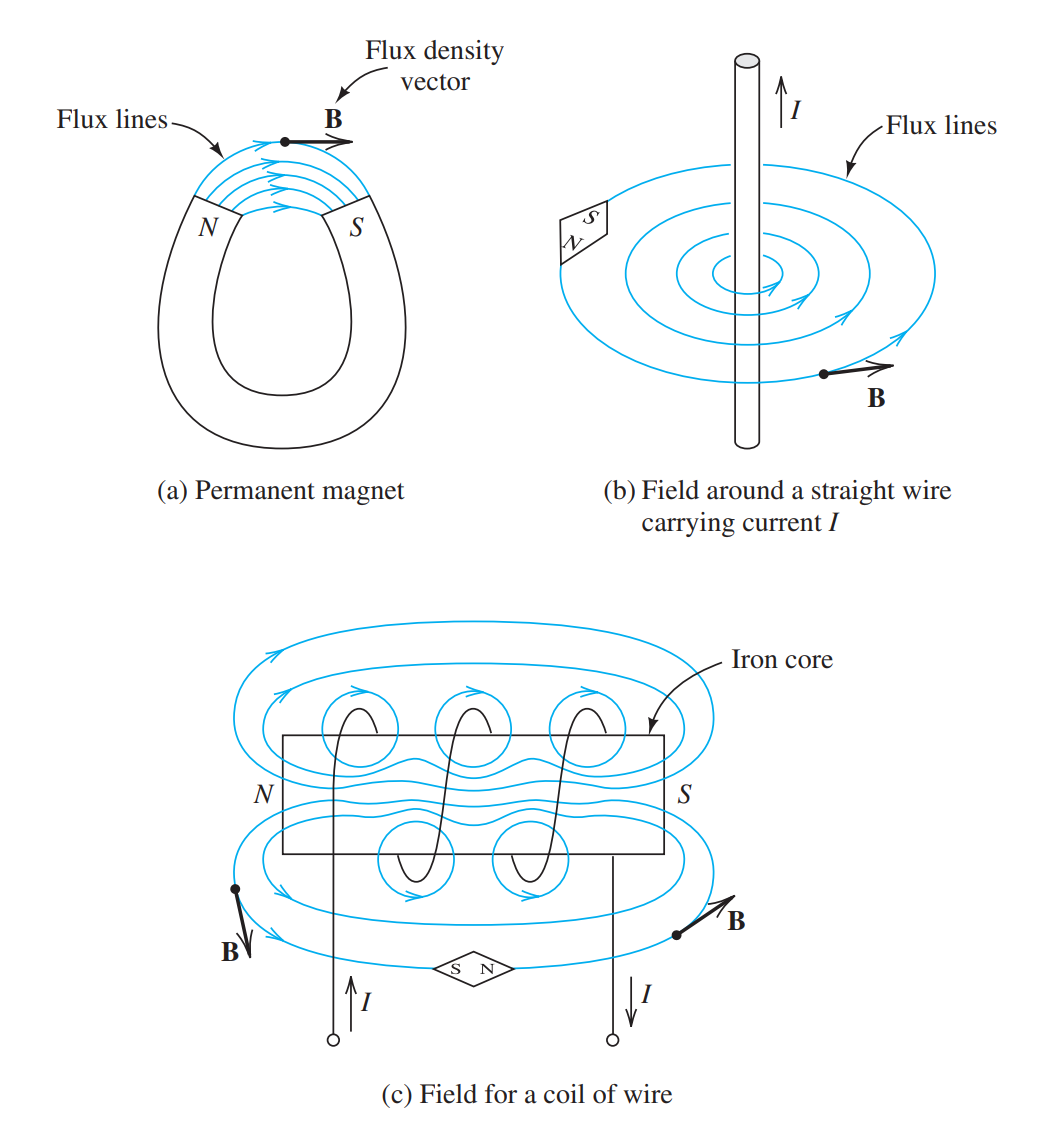
\includegraphics[width=0.4\linewidth]{images/magnetic-fields-lines.png}
    \caption{Magnetic fields can be visualized as lines of flux that form closed paths. Using a compass, we can determine the direction of the flux lines at any point. Note that the flux density vector $\symbfit{B}$ is tangent to the lines of flux.}
    \label{fig:magnetic-fields-lines}
\end{figure}
The units of magnetic field are webers. ($Wb$)
\begin{notebox}
    \begin{remark}
        Note that Flux lines leave the north-seeking end of a magnet and enter the south-seeking end.
    \end{remark}
\end{notebox}
\subsubsection{Magnetic Flux Density}
In equations, we represent the \textbf{magnetic flux density} as the vector quantity $\symbfit{B}$ and its corresponding lightface italic symbol $\textit{B}$ as the magnitude of the vector $\symbfit{B}$. The units of $\symbfit{B}$ are $webers/{meter}^2$ ($Wb/m^2$) or, equivalently, teslas ($\symbfit{T}$). The flux density vector $\symbfit{B}$ has a direction tangent to flux lines, as illustrated in Figure \ref{fig:magnetic-fields-lines}.
\subsection{Right-Hand Rule}
The direction of the magnetic field produced by a current can be determined by the right-hand rule. There are two interpretations of this rule.
\begin{enumerate}
    \item As illustrated in Figure \ref{fig:right-hand-rule-1}, if a wire is grasped with the thumb pointing in the direction of the current, the fingers encircle the wire, pointing in the direction of the magnetic field.
    \begin{figure}[H]
        \centering
        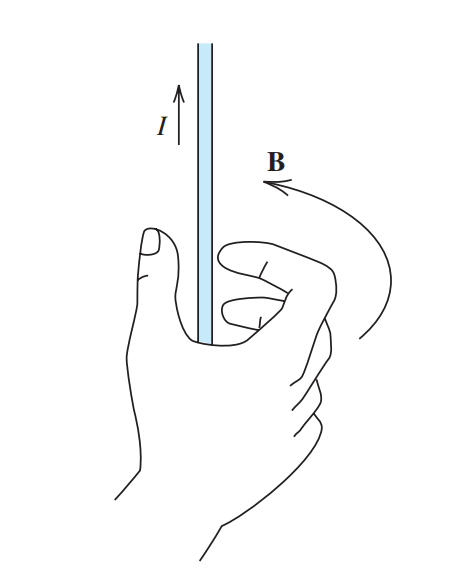
\includegraphics[width=0.3\linewidth]{images/right-hand-rule-1.png}
        \caption{Illustration 1}
        \label{fig:right-hand-rule-1}
    \end{figure}
    \item Moreover, as illustrated in \ref{fig:right-hand-rule-2}, if the fingers are wrapped around a coil in the direction of current flow, the thumb points in the direction of the magnetic field that is produced inside the coil.
    \begin{figure}[H]
        \centering
        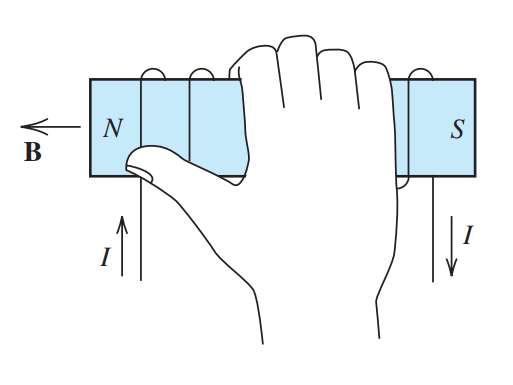
\includegraphics[width=0.3\linewidth]{images/right-hand-rule-2.png}
        \caption{Illustration 2}
        \label{fig:right-hand-rule-2}
    \end{figure}
\end{enumerate}
\subsection{Forces on Charges Moving in Magnetic Fields}
An electrical charge $q$ moving with velocity vector $\symbfit{u}$ through a magnetic field $\symbfit{B}$ experiences a force $\symbfit{f}$ as illustrated in Figure \ref{fig:forces-on-moving-charges-in-magnetic-fields}. The force vector is given by,
\begin{equation} \label{eq: force-vector}
    \symbfit{f} = q\symbfit{u} \times \symbfit{B}
\end{equation}
in which $\times$ represents the cross product. Because of the definition of cross product, we can know the magnitude of the force is given by
\begin{equation} \label{eq: force-vector-magnitude}
    f=quB~sin(\theta)
\end{equation}
in which, $\theta$ is the angle between $\symbfit{u}$ and $\symbfit{B}$, as illustrated in the figure \ref{fig:forces-on-moving-charges-in-magnetic-fields}.
\begin{figure}[H]
    \centering
    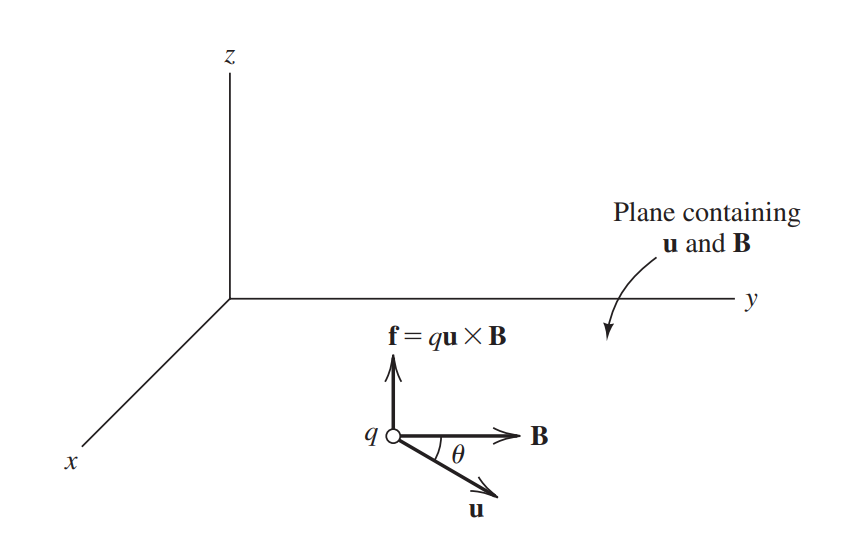
\includegraphics[width=0.5\linewidth]{images/forces-on-moving-charges-in-magnetic-fields.png}
    \caption{Forces on charges moving in magnetic fields}
    \label{fig:forces-on-moving-charges-in-magnetic-fields}
\end{figure}
\begin{notebox}
    \begin{remark}
    Note that
    \begin{enumerate}
        \item Force is exerted on a charge as it moves through a magnetic field.
        \item In the force vector equation \eqref{eq: force-vector}, the charge $q$ can be negative, which will opposite the direction of the vector.
        \item In the magnitude of force vector equation \eqref{eq: force-vector-magnitude}, we always treat the charge $q$ to have no signs.
    \end{enumerate}
        
    \end{remark}
\end{notebox}
\end{document}
